\documentclass[12pt]{article}

\usepackage{sbc-template}
\usepackage{graphicx,url}
\usepackage[utf8]{inputenc}
\usepackage[brazil]{babel}
%\usepackage[latin1]{inputenc}
\usepackage{listings}
\usepackage{multicol}

\sloppy

\title{Arquitetura Genérica para Processamento de Eventos em Streaming utilizando Apache Kafka}

\author{Jânio P. Otoni\inst{1}, Evandrino G. Barros\inst{1}, Anolan Milanes\inst{2}}
\address{
Departamento de Computação\\ Centro Federal de Educação Tecnológica de Minas Gerais (CEFET-MG)\\ 30.510-000 -- Belo Horizonte -- MG -- Brasil
\nextinstitute
  Faculty of Logistics -- Molde University College\\
  6402 -- Molde -- NO
\email{academic@janio.dev, evandrino@cefetmg.br, anmi@himolde.no}
}

\begin{document} 

\maketitle

\begin{abstract}
  The intention of this article is to describe, in a theoretical and practical way, a data processing architecture that is able to process data generated by IoT devices positioned in forest regions of environmental preservation in a continuous way. Through concepts of databases and distributed systems, and big data techniques we seek to create a resilient and highly available system capable of detecting the onset of a fire through the regular events carried out by the devices connected to the network.
\end{abstract}
     
\begin{resumo} 
  A intenção deste artigo é descrever, de forma teórica e prática, uma arquitetura de processamento de dados que seja capaz de processar dados através de uma arquitetura de processamento em streaming que seja de fácil replicação. Trabalhando em cima de exemplos de uso para IoTgerados por dispositivos de internet das coisas posicionados em regiões florestais de preservação ambiental de forma contínua. Através de conceitos de bancos de dados e sistemas distribuídos, e técnicas de \textit{big data} buscamos criar um sistema resiliente e com alta disponibilidade capaz de detectar o início de um incêndio através dos eventos regulares realizados pelos dispositivos conectados em rede.
\end{resumo}



\section{Introdução}
Processar dados em \textit{streaming} nos permite pensar na natureza e comportamento dos dados, para processá-los como se fossem um sinal digital em que conhecendo os padrões de recorrência dos dados, somos capazes de manipular esta informação de forma a detectar padrões de comportamento e aplicar funções que modifiquem o estado do sistema conforme novos eventos são emitidos para o sistemas.

Pense, como um exemplo, em um sistema de detecção de incêndios florestais. Dentro da floresta, são posicionados sensores de temperatura para detectar variações bruscas de temperatura para identificar focos de incêndio. Como a direção do vento pode variar, imagine que é feito um arranjo com triangulação, em que três sensores ficam próximos e a informação dos três precisa ser levada em consideração para uma tomada de decisão, como disparar um alarme de incêndio. E isto precisa ser feito em tempo real, pois um foco de incêndio pode rapidamente se tornar incontrolável.

Um sistema de processamento em \textit{streaming} pode ser ideal para esse tipo de problema (\cite{isah:18} e \cite{meehan:17}), e diversos outros em que os dados precisam ser processados com baixa latência ou os dados que são tratados possuem uma recorrência temporal, ou são analisados e agregados à medida que novas informações sobre o estado do sistema são despachadas. Claro que estes sistemas não são perfeitos e uma infinidade de problemas podem ocorrer em decorrência do alto volume de dispositivos e dados, porém podem ser contornados escalando o sistema, ao custo de mais máquinas de processamento \cite{dey:18}. E isto vai de encontro com o problema apresentado anteriormente! Neste tipo de sistema os dados são processados de forma assíncrona e com baixíssima latência (próximo ao tempo real) à medida em que esses novos eventos publicam novas mensagens.

Com a a preservação ambiental se destacando nas pautas políticas, inclusive gerando conflito entre governos ao redor do mundo, este assunto se torna cada vez mais importante. Como o controle de incêndios é um desafio para as autoridades brasileiras dada a escassez de recursos humanos e técnicos para o controle de grandes incêndios, a detecção precoce é o melhor caminho para se evitar tais danos ambientais.

Um sistema de monitoramento de internet das coisas pode representar uma forma eficiente e barata de realizar esse tipo de monitoramento \cite{albuquerque:20}, porém a limitação computacional dos dispositivos empregados em campo e a necessidade de centralização dessas informações para a tomada de decisão, cruzamento de informações e alarmes em tempo real e é neste momento em que as coisas se combinam e se torna interessante propor um sistemas do tipo para a tratativa deste problema.

O objetivo deste trabalho é, então, servir como proposta de tratamento dos dados gerados por dispositivos de internet das coisas para o \textbf{Grupo de Detecção e Controle à Incêndios} do Departamento de Computação do CEFET-MG. O fluxo de dados do sistema começa nos detectores e é servido ao sistema através de um \textit{broker} MQTT, que é colocado em um \textit{stream} de dados e processado por uma plicação de onde são retiradas informações de visualização do estado do sistema (medidas de temperatura, umidade, luminescência e gases inflamáveis) e disparo de alarmes quando alguma dessas medidas ou o conjunto delas acusarem o foco de um incêndio.
 


\section{Referencial Teórico}
\subsection{Arquitetura Direcionada a Eventos}
Uma arquitetura de software direcionada a eventos produz, detecta, consome e reage a eventos. Um evento é uma mudança de estado do sistema, que quando ocorre, produz uma mensagem (notificação de evento) de forma assíncrona que é publicada, propagada pelo sistema, detectada e consumida por outro componente/serviço. É uma abordagem ideal para o desenvolvimento de sistemas de baixo acoplamento, em que os componentes ou serviços conhecem muito pouco ou nada sobre os demais componentes do sistema.

Um sistema orientado a eventos possui no mínimo três atores: emissores de eventos, que transfere eventos e não sabe se existe consumidor para esse evento e tampouco como ele lida com essa notificação e evento; coletores de eventos, que reagem assim que detectam uma notificação de evento, que pode ser a execução de uma tarefa ou uma nova mudança de estado que será propagada novamente pelo sistema; e canais de eventos, que são onde emissores e consumidores se conectam para emissão e consumo de notificações de mudança de estado.

\subsection{Programação reativa}
Programação reativa é um modelo declarativo assíncrono, não-bloqueante e direcionado a eventos. Os \textit{threads} que compartilham recursos não são bloqueados aguardando por recursos, eles fazem um \textit{request}, continuam a execução e são notificados quando a atividade acabou de ser realizada. Essas características podem ser alcançadas através de três métodos: futuros/promessas, \textit{streams} reativas (fluxos de dados sem limites) e variáveis de fluxo (memória compartilhada). A grosso modo, programação reativa é aplicação do modelo \textit{pub/sub} em uma linguagem de programação. Um \textit{publisher} gera um evento e um \textit{subscriber} o lê.

\subsection{Processamento em \textit{streaming}}
Processamento em streaming é um termo praticamente análogo a programação reativa, porém, quando utilizado, costuma ter o intuito de realçar as características de tempo de um sistema. Podemos pensar como sistemas que processam um fluxo de dados “sem começo e nem fim”, que visa responder a eventos com a menor latência possível, e geralmente utiliza o tempo como parâmetro para agregação e transformação dos dados. Ele pode ser entendido como uma generalização de processamento em batch, que acumula um grande volume de dados, por um longo período de tempo, e processa tudo de uma vez (aumentando o throughput e a latência drasticamente). É uma boa escolha quando a natureza do dado é ser publicada em um fluxo de dados sem fim, quando os resultados do processamento devem ser publicados o mais rápido possível ou quando o volume é tão grande que não pode ser armazenado.




\subsection{Apache Kafka}

A Kafka é uma plataforma de processamento de eventos em \textit{streaming} que tem um papel central para a construção da arquitetura proposta. Dado a sua importância para o projeto, decidimos por explicar da melhor maneira possível seu funcionamento e principais conceitos.

O \textit{log} é o conceito mais fundamental da Kafka. No ponto de vista dos desenvolvedores da Kafka, esse sistema que muitas vezes é entendido como um sistema orientados a mensagens (como o \textit{RabbitMQ}) possui suas raízes em ideias muito diferentes. Ele pode ser pensado como um “banco de dados de dados de cabeça para baixo”, pois a unidade mais fundamental de um banco de dados moderno é justamente seu \textit{log} de transações, que fica oculto do usuário, e só é acessado através de \textit{queries}. Estes \textit{logs} são acrescentados de uma forma \textit{append only}, o que garante performance, escalabilidade e imutabilidade dos dados.

Dando um passo adiante, estes logs costumam ser organizados como um conjunto chave/valor. Essa chave costuma carregar os metadados de uma linha do banco, que são necessários para encontrar e acessar algum conjunto de informações. Por sua vez, por questões de otimização de acesso e espaço, os valores relacionados a uma chave se encontram em um formato serializado o qual o banco é capaz de deserializar, e como ele é algo bem específico do banco, não há um protocolo público de acesso direto a esses dados. A Kafka “expõe seu” e \textit{log} e fornece serializadores/deserializadores que permite às aplicações produtoras ou consumidoras a compreender os dados presentes nos \textit{logs}. Estes serializadores podem, inclusive, ser criados pelo próprio usuário, o tornando extremamente flexível e independente de um protocolo de comunicação a nível de aplicação.

Quando tratamos da exposição desta estrutura para o usuário, é importante entender o que são: produtores (são as aplicações que geram eventos), consumidores (as aplicações que consomem eventos), \textit{brokers} (os nós de computação em um \textit{cluster} que serve à Kafka) e tópico (a unidade de informação que concentra eventos do mesmo tipo, é alimentado por produtores e é onde os consumidores recebem notificações e leem novos eventos).

Para garantir alta resiliência e disponibilidade, o ideal é que um \textit{cluster} de Kafka possua no mínimo três \textit{brokers}. Também é desejado que este \textit{cluster} seja homogêneo, para garantir o balanceamento adequado entre os nós. Voltando aos tópicos, eles são materializados através de partições, que são distribuídas pelo \textit{cluster}. Estas partições podem ser escaladas de 1 a N, e cada partição terá 1/N das informações de um tópico. Esse N também é importante, pois, ele também representa o número de consumidores que consumir informações deste tópico dentro de um mesmo grupo.

Um consumidor se cadastra em um tópico e consome dados de uma ou mais partições. Um grupo de consumidores é o conjunto de N (número de partições no tópico) ou menos aplicações consumidoras idênticas, que são escaladas horizontalmente. Dentro do mesmo grupo, cada tópico só pode ser associado a um consumidor (para evitar a leitura duplicada de eventos), porém o número de grupo de consumidores associados a um tópico, consumindo dados simultaneamente dos mesmos tópicos é virtualmente infinito. Porém, um grupo de consumidores é completamente isolado do outro, sendo as garantias de processamento e ordem dos eventos relacionadas apenas dentro de cada grupo individualmente. Um esquema de como é a operação da Apache Kafka é apresentado na Figura~\ref{fig:kafkaCluster}, este exemplo visa apresentar uma simplificação da organização de um \textit{cluster} que serve a diversas aplicações, o desacoplamento entre elas e a relação entre \textit{brokers}, tópicos e partições. Arranjos mais complexos podem ser criados, mas por simplicidade escolhemos descrever um \textit{cluster} simplificado.

\begin{figure}[ht]
    \centering
    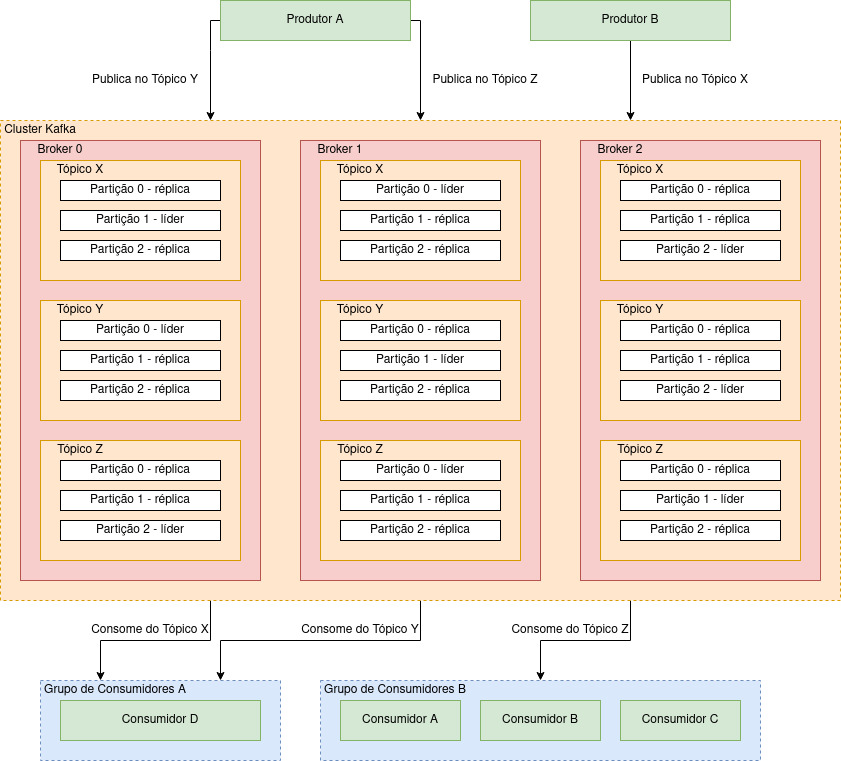
\includegraphics[width=0.8\textwidth]{images/kafkaCluster.jpg}
    \caption{\textit{Cluster} Kafka - ilustração de operação de um conjunto de aplicações através da Kafka. Note que não há relação alguama entre produtores e consumidores.}
    \label{fig:kafkaCluster}
\end{figure}

Estas características tornam a Kafka extremamente escalável, e permite às aplicações que utilizam sua infraestrutura escaláveis também, e por ter uma proposta centrada em dados, apenas seu estado precisa ser preservado, permitindo às demais aplicações (produtores/consumidores) serem \textit{stateless}. Porém, outras aplicações apresentam características semelhantes, e um grande trunfo da Kafka em sua concepção foi a persistência. Diferente de sistemas de mensagens, os eventos na Kafka são persistidos em suas partições por um período configurável, e diferente de um sistema em que as mensagens são consumidas e deletadas imediatamente da fila, aos eventos de uma partição são atribuídos \textit{offsets} que permitem ao \textit{broker}/consumidor controlar a última posição lida de uma partição. Isso elimina um problema de sistemas \textit{pub/sub} denominado \textit{backpressure}, que ocorre quando a taxa de produção de mensagens/eventos é muito maior que a taxa de consumo dessa informação, levando a perda de dados, uma vez que o dados é persistido e pode ser produzido/consumido com diferentes taxas.

Além de tudo já citado, o que torna a Kafka uma plataforma, são seus conectores e bibliotecas de processamento em \textit{stream}. A biblioteca de processamento é uma \textit{API} Java que simplifica o desenvolvimento de aplicações que fazem o uso da Kafka para o processamento de dados. A \textit{Connect API} permite criar conectores que integram outros sistemas/aplicações à Kafka. Juntando todas as partes (conectores / processamento em \textit{stream} / persistência / \textit{logs}) a Kafka é em si um sistema completo de processamento de dados, abrangendo todo os espectro de coleta, transporte, processamento e armazenamento de dados.

Quanto à infraestrutura, a Kafka demanda o \textbf{Apache ZooKeeper}. Ele é um cluster de serviço que visa prover "coordenação distribuída altamente confiável" para aplicações. Essencialmente, ele é um programa distribuído que oferece um sistema de bancos de dados chave-valor hierárquico. Isto quer dizer que ele organiza suas informações de uma forma semelhante a uma árvore, em que cada nó aponta para um conjunto de informações utilizada pelas aplicações distribuídas para serviço de configuração, nomeação e sincronização das mesmas.

\subsubsection{Processamento Transacional}

As garantias de processamento no Kafka servem para atender a diferentes tipos de cargas de trabalho. A decisão por uma delas impacta diretamente na confiabilidade e desempenho do sistema. De forma simplificada, quanto menor as garantias, menor a quantidade de checagens que o sistema precisa realizar ara garantir a integridade do sistema, o que resulta em maior desempenho e menor tolerância a falhas.

\textbf{Nenhuma Garantia}: até então, esta é  configuração padrão do Kafka. Quando não são especificadas as devidas configurações, não há nenhum tipo de garantia, as mensagens podem ser tanto duplicadas quanto perdidas. Este é o modo em que o sistema apresenta a maior vazão, porém, é o modo de operação de menor confiabilidade.

\textbf{No máximo uma vez (melhor esforço)}: Com esta configuração

\textbf{Pelo menos uma vez}

\textbf{Exatamente uma vez}
Escritas idempotentes
Transações
Salvar progresso e dados atomicamente


\section{Infraestrutura}
\subsection{Contêiner}
Para entender o Docker, precisamos primeiro entender o que é um contêiner.Um \textbf{contêiner} é uma unidade de software padronizada que empacota o código e todas as suas dependências (\textit{runtime}, ferramentas e bibliotecas de sistema, e configurações), assim, desacoplando a aplicação da infraestrutura, permitindo sua implementação em diversos ambientes diferentes, sendo executados da mesma forma em diferentes configurações. Além disso, um contêiner é extremamente leve por utilizar o \textit{kernel} do Sistema Operacional da máquina, não sendo necessário a criação de uma máquina virtual por aplicação, e o torna ótimo para desenvolvimento também, uma vez que o desenvolvedor tem o controle do ambiente da aplicação e ela executará da mesma forma em produção. Por fim, essa maneira de empacotar aplicações gera desacoplamento e isolamento das aplicações, tornando o ambiente mais segura.

Para que um contêiner possa rodar em um dado Sistema Operacional, ele precisa de um serviço que intermedeie a comunicação com o SO, e em nosso caso, a \textbf{Docker Engine} é responsável por isso. Por ter sido desenvolvido inicialmente para Linux, ele faz o uso do \textit{cgroups} (\textit{control groups} - recurso que limita, contabiliza e isola recursos como CPU, memória, I/O, rede, para grupos de processos) e \textit{namespaces} (recurso que particiona os recursos do \textit{kernel} de modo que um conjunto de processos veja um conjunto de recursos enquanto outro conjunto de processos vê um conjunto diferente de recursos).

\subsection{Docker}
A \textbf{Docker} é uma plataforma para desenvolvimento, distribuição e execução de aplicações. Ela permite o desacoplamento entre aplicação e infraestrutura e agiliza a entrega de software ao empacotar todo o software e suas dependências em uma imagem capaz de rodar sobre o \textit{kernel} do Linux, isolando a aplicação sem que seja necessário a criação de máquinas virtuais pada cada aplicação, economizando recursos e extraindo mais desempenho.

Sua arquitetura é do tipo cliente-servidor, que se comunicam através de uma API REST. Isto permite o desacoplamento entre o cliente e o \textit{daemon}, permitindo que o cliente envie comando tanto a um \textit{daemon} local quanto remoto. além destes componentes, ainda existe o \textit{registry}, que é um servidor que pode ser configurado como repositório, no qual diversos Docker \textit{daemons} podem publicar e baixar imagens. Em resumo, a Docker é capaz de gerenciar imagens, volumes de dados, redes e contêineres para o pleno funcionamento dessas aplicações.

%\begin{figure}[ht]
%\centering
%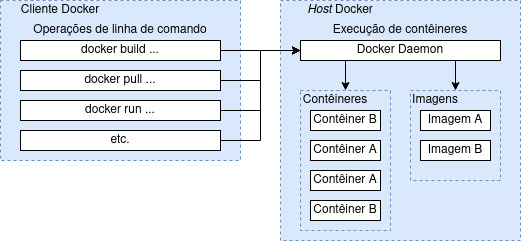
\includegraphics[width=0.8\textwidth]{images/docker.jpg}
%\caption{Docker}
%\label{fig:docker}
%\end{figure}

\textbf{Docker Swarm} é um orquestrador de contêineres que facilita o trabalho de distribuir imagens e gerenciar serviços através de um \textit{cluster}. Cada maquina que integra o Swarm pode ser um \textbf{nó} \textit{manager} ou \textit{worker}, sendo que um nó de gerenciamento pode também atuar como trabalhador (executando contêineres). Para se realizar o \textit{deploy} de uma aplicação no Swarm é necessário enviar uma \textit{stack} para um nó manager, que é uma especificação de um \textbf{serviço}, onde são declaradas replicação, variáveis de ambiente, configurações, segredos, quantidade de CPU, memória RAM, redes, etc. Assim, os nós de trabalhadores recebem \textbf{tarefas}, que nada mais são que um contêiner que deve ser executado conforme as especificações definidas pelo serviço. Outro componente importante do Swarm é o \textbf{balanceamento de carga}, que permite que aplicações externas acessem o \textit{cluster} através da exposição das portas especificadas pelo serviço. A Figura~\ref{fig:swarmCluster} descreve como é o arranjo de um \textit{cluster} Swarm e a interação entre os nós. Por servir como uma camada de isolamento, Ele nos permite operar com diversas versões da mesma aplicação e distribuir as tarefas de forma simples entre os nós.

\begin{figure}[ht]
    \centering
    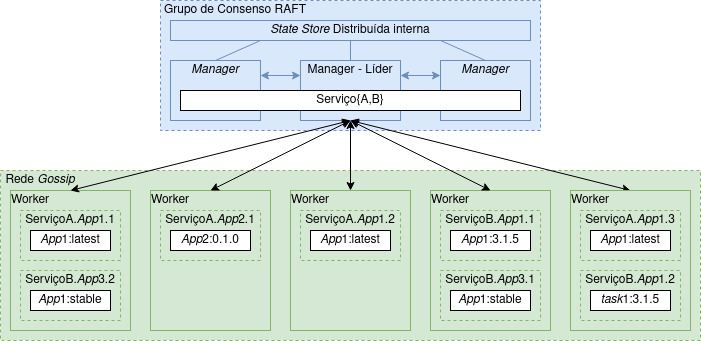
\includegraphics[width=0.8\textwidth]{images/swarmCluster.jpg}
    \caption{\textit{Cluster} Docker Swarm - Organização e correlação entre nós}
    \label{fig:swarmCluster}
\end{figure}




\subsection{Infraestrutura na Nuvem}
A infraestrutura na nuvem é uma quebra de paradigma em que as empresas e instituições de diversas orientações abrem mão de manter uma infraestrutura local de servidores, para contratá-los como um serviço. Isto é interessante, pois, ao invés de manter uma infraestrutura local que é difícil de manter e pode rapidamente se tornar obsoleta, os clientes têm acesso a um serviço co altíssima disponibilidade. %incluir referência a CA Patterson

Com o passar do tempo, essas empresas que ofereciam serviços simples de hospedagem de máquinas virtuais online, passaram a enriquecer sua prateleira de serviços, e uma série de novas práticas e ferramentas foram desenvolvidas para simplificar a operação desses serviços. Novos recursos e serviços são adicionados constantemente pelos fornecedores e diversos deles foram utilizados neste trabalho. %levantar dados históricos

\subsubsection{Oracle Cloud Infrastructure - OCI}
A OCI é o serviço de computação em nuvem da Oracle. Assim como em outros provedores, ela fornece diversos recursos de armazenamento, processamento e rede necessários para a construção e escala dos mais diversos tipos de serviços. Ela possui um plano que oferece recurso grátis dentro de uma limitação que é bem razoável e que nos permite desenvolver algumas aplicações distribuídas sem custos e validar diversos conceitos, como os apresentados neste trabalho.

\subsubsection{Infraestrutura como Código}
A infraestrutura como código (IaC) usa uma linguagem de codificação descritiva de alto nível para automatizar o provisionamento de infraestrutura de TI. Essa automação elimina a necessidade dos desenvolvedores de provisionar e gerenciar manualmente servidores, sistemas operacionais, conexões de banco de dados, armazenamento e outros elementos de infraestrutura sempre que desejam desenvolver, testar ou implantar um software.

A IaC permite a criação e versionamento de infraestruturas rapidamente da mesma forma que versionam o código-fonte e rastreiam essas versões para evitar inconsistências entre os ambientes de TI que podem levar a sérios problemas durante a implantação e garante que a mesma infraestrutura pode ser sempre reproduzida.




\section{Formato de Dados}
\subsection{Avro}
A adoção de esquemas de dados favorece a construção de um sistema complexo por exigir um contrato de dados para que todos os sistemas interessados no processamento de tal informação seja capaz de reconhecer o mesmo padrão de dados. Além disso, por definirem um padrão que possibilita a serialização de dados, é possível armazenar os dados de forma mais compacta para que ele seja transmitido e reconstruído de forma mais eficiente. O formato Avro foi escolhido para esse projeto por ser, dentre os padrões de serialização mais adotados hoje em dia, o mais maduro, com suporte nativo a evolução de esquemas, sua melhor integração com o Kafka e facilidade de gerar código para diferentes linguagens de gramação a partir dos próprios esquemas.

Avro é um formato RPC (remote procedure call) e um framework dentro do ambiente do Apache Hadoop (um conjunto de ferramentas de código aberto que facilitam a utilização de clusters de computadores para o processamento de quantidades massivas de dados – Big Data). Ele utiliza JSON para a definição dos tipos de dados e protocolos, e serializa os dados em um formato binário compacto. Os blocos de dados podem ser codificados: em formato binário, adotado pela maioria das aplicações por ser menor e mais rápido ou em formato JSON, para depuração ou aplicações web. Outro aspecto importante é que um arquivo avro pode vir ou não com o esquema de dados presente em seu cabeçalho.

Os esquemas são definidos usando JSON, seus tipos primitivos são: 
\begin{center}
    \begin{tabular}{ |c|c|c| }
        \hline
        TIPO    & DESCRIÇÃO                                                 & EXEMPLO \\
        \hline
        null    & nenhum valor                                              & null \\
        boolean & um valor binário                                          & true \\
        int     & inteiro com sinal de 32 bits                              & 1 \\
        long    & inteiro com sinal de 64 bits                              & 1 \\
        float   & ponto flutuante IEEE 754 de precisão simples (32 bits)    & 1.1 \\
        double  & ponto flutuante IEEE 754 de precisão dupla (64 bits)      & 1.1 \\
        bytes   & sequência de bytes sem sinal de 8 bits                    & “\textbackslash u00FF” \\
        string  & sequência de caracteres unicode                           & “foo” \\
        \hline
    \end{tabular}
%\caption{\label{tab:table-name}Your caption.}
\end{center}

e seus tipos complexos são: record, enum, array, map, union e fixed. Os utilizados neste projeto são:

\subsubsection{Unions}

As uniões são representadas por meio de matrizes JSON. Por exemplo, ["null", "string"] declara um esquema que pode ser nulo ou string. Uniões não podem conter imediatamente outras uniões. (Observe que quando um valor padrão é especificado para um campo de registro cujo tipo é uma união, o tipo do valor padrão deve corresponder ao primeiro elemento da união. Assim, para uniões contendo "nulo", o "nulo" geralmente é listado primeiro, uma vez que o valor padrão de tais uniões é normalmente nulo.)

\subsubsection{Records}
Os registros usam o nome de tipo "record" e oferecem suporte aos seguintes atributos: 

\begin{itemize}
    \item \textbf{name} (obrigatório): uma string JSON fornecendo o nome do registro;
    
    \item \textbf{fields} (obrigatório): uma matriz JSON, campos de listagem. Cada campo é um objeto JSON com os seguintes atributos: 
    \begin{itemize}
        \item \textbf{name} (obrigatório): uma string JSON fornecendo o nome do campo;
        
        \item \textbf{doc} (opcional): uma string JSON que descreve este campo para usuários;
        
        \item \textbf{type} (obrigatório): um esquema, conforme definido acima;
        
        \item \textbf{default} (opcional): um valor padrão para este campo, usado apenas ao ler instâncias que não possuem o campo para fins de evolução do esquema. A presença de um valor padrão não torna o campo opcional no momento da codificação. Os valores permitidos dependem do tipo de esquema do campo. Os valores padrão para campos de união correspondem ao primeiro esquema na união. Os valores padrão para bytes e campos fixos são strings JSON, em que os pontos de código Unicode 0-255 são mapeados para valores de byte de 8 bits não assinados 0-255. Avro codifica um campo mesmo se seu valor for igual ao padrão;
        
        \item \textbf{order} (opcional): especifica como este campo afeta a ordem de classificação deste registro. Os valores válidos são "ascendente" (o padrão), "descendente" ou "ignorar";
        
        \item \textbf{aliases} (opcional): uma matriz JSON de strings, fornecendo nomes alternativos para este campo.
    \end{itemize}
    
    \item \textbf{namespace} (opcional): uma string JSON que qualifica o nome;
    
    \item \textbf{doc} (opcional): uma string JSON que fornece documentação ao usuário deste esquema;
    
    \item \textbf{aliases} (opcional): uma matriz JSON de strings, fornecendo nomes alternativos para este registro.
\end{itemize}

Por exemplo, uma lista de medidas de um detector pode ser definida com:
\begin{lstlisting}
{ 
  "type": "record", 
  "name": "DetectorV3",
  "aliases": [ "DetectorV1", "DetectorV2" ],
  "fields" : [ 
    { "name": "MedidaA", "type": "long" },
      { "name": "MedidaB", "type": [ "null", "long" ] }
  ] 
}
\end{lstlisting}

Um esquema nada mais é que a definicao de como os dados devem ser organizados, e devem ser escritos pelo administrador/desenvolvedor dos sistemas. Diferente de um arquivo CSV, por exemplo, um formato de registro pode ser predefinido e conhecido a priori. Como exemplo, podemos pegar um trecho com duas linhas de dados retirados do dataset utilizado nesse projeto:

\begin{center}
    \begin{tabular}{ |c|c|c|c|c|c|c|c|c|c|c|c|c| }
        \hline
        X	& Y & month	& day	& FFMC	& DMC	& DC	& ISI	& temp	& RH	& wind	& rain	& area  \\
        \hline
        7	& 5	& mar	& fri	& 86.2	& 26.2	& 94.3	& 5.1	& 8.2	& 51	& 6.7	& 0	    & 0     \\
        7	& 4	& oct	& tue	& 90.6	& 35.4	& 669.1	& 6.7	& 18	& 33	& 0.9	& 0	    & 0     \\
        \hline
    \end{tabular}
\end{center}

E a partir das informações apresentadas, podemos criar um esquema que será utilizado por todos os programas envolvidos na produção, transporte e consumo destes dados:

\begin{lstlisting}[]
{
  "namespace": "dev.janio", 
  "type": "record", 
  "name": "forestfires", 
  "doc": "Esquema utilizado para descrever os dados
          coletados por um conjunto de dispositivos
          para a deteccao de incendios.", 
  "fields": [ 
    { "name": "X",     "type": ["null", "int"]    }, 
    { "name": "Y",     "type": ["null", "int"]    }, 
    { "name": "month", "type": ["null", "string"] }, 
    { "name": "day",   "type": ["null", "string"] }, 
    { "name": "FFMC",  "type": ["null", "float"]  }, 
    { "name": "DMC",   "type": ["null", "float"]  }, 
    { "name": "DC",    "type": ["null", "float"]  }, 
    { "name": "ISI",   "type": ["null", "float"]  }, 
    { "name": "temp",  "type": ["null", "float"]  }, 
    { "name": "RH",    "type": ["null", "int"]    }, 
    { "name": "wind",  "type": ["null", "float"]  }, 
    { "name": "rain",  "type": ["null", "float"]  }, 
    { "name": "area",  "type": ["null", "float"]  } 
  ]
}
\end{lstlisting}

\section{Trabalhos Relacionados}
Já existem esforços para a utilização de sistemas de \textit{streaming} para o processamento de dados de forma genérica, em sua maioria, visam utilizar a maior quantidade de poder computacional e armazenamento de dados para esse tipo de processamento. Quando um sistema possui restrições de tempo muito severas, a integração entre os sistemas se torna crucial e diversas manobras para os serviços de dados são adotados, para garantir o acesso à informação o quanto antes, em diferentes estágios do \textit{pipeline} de processamento \cite{isah:18}.

Diferente de sistemas de processamento em \textit{batch}, como os \textit{Data Warehouses}, sistemas de processamento em \textit{streaming} requerem a capacidade de lidar com registros fora de ordem e perdidos, a ordem de execução do fluxo de dados (atingido através de \textit{DAGs}) e a garantia de processar exatamente uma vez cada registro que entre no fluxo de processamento. Em questão de infraestrutura, ele deve ser capaz de armazenar arquivos localmente, garantir que as transações atendam às propriedades \textit{ACID}, seja escalável e entregue os dados mais recentes com baixa latência. Os componentes básicos de um sistema de \textit{streaming} são um coletor, ingestor, processador analítico e uma ferramenta de migração de dados \cite{meehan:17}.

Diferentes topologias para a organização dos dados podem ser adotadas e elas podem ter um impacto significativo na performance do sistema. Uma topologia com granularidade menor, em que cada dispositivo é disposto em seu próprio tópico leva a maior desempenho do sistema, porém a um custo computacional mais elevado e maior necessidade de escalar o sistrema. Para manter o sistema a baixo custo, sem a necessidade de dispor de muitas máquinas, o ideal pode ser de arranjar os dados de maneira agrupada antes de disponibilizá-los para análise, poupando processamento, e evitando possíveis problemas de latência \cite{dey:18}.

\subsection{Sistema de Internet das Coisas para Detecção de Incêndios Florestais}
Os sistemas baseados em \textit{IoT} possuem uma das maiores relações custo benefício com relação a detecção, manutenibilidade e tempo de resposta aos incêndios. A utilização de se sensores baratos e a boa seleção de características a serem analisadas podem levar o sistema a apresentar ótimos resultados na detecção e prevenção de incêndios. Fatores limitantes são o tamanho vasto da área monitoramento, escassez de recursos energéticos e a dificuldade de se alcançar as regiões onde os sensores devem ser posicionados, fora o risco de os próprios detectores de incêndio correrem o risco de serem incinerados durante uma queimada \cite{albuquerque:20}.

A adoção de um sistema de internet das coisa para a detecção e prevenção de incêndios possui um apelo muito forte, devido à sua alta conectividade e baixo custo quando comparado a sistemas mais robustos. Porém, existe uma série de desafios que devem ser encarados para a tratativa dos dados gerado por estes dispositivos. Como são construídos pensados em baixo custo e consumo energético para se manterem ligados em cenários com grande restrição de recursos, o formato de dados gerados por tais dispositivos se torna fundamental para a operação adequada do sistema.

Para a economia de recursos de rede, energia e processamento, é ideal que este formato de dados seja serializado em um formato binário, reduzindo o tráfego de dados e por consequência o consumo energético dos dispositivos. Porém, dados binários podem ser complicadores, uma vez que eles devem ser tratados em algum ponto do sistema para a realização de análise sobre esses dados. Assim, um aspecto fundamental tanto para o sistema de captura e transporte de dados sobre incêndio quanto para o sistema de processamento desses dados é que haja um "contrato", que reforce o formato de dados e seja compreendido de ponta a ponta do sistema.

Existem diversos formatos de serialização de dados, entre formatos binários e textuais e para garantir essa integração e o alto desempenho do sistema, escolhemos trabalhar com o formato Avro. A ideia se apoia em um primeiro facilitador, que é fato de o Avro ser um formato de serialização nativo para a Apache Kafka, o que facilita o seu processamento. Muito além disso, Avro é o formato de serialização mais utilizado em \textit{big data} para o transporte de dados, é um formato mantido pela Apache Foundation (o que garante neutralidade), possui um esquema que pode ser utilizado para a definição do formato do dado em todo o \textit{pipeline}, pode ser serializado/deserializado em binário e JSON, e possui uma especificação que torna os binários extremamente compactos.

\section{Experimentos}

\subsection{Contexto/Ambiente}
Os testes para o sistema foram projetados para serem executados no ambiente da OCI. Foram empregadas quatro máquinas virtuais com a configuração de 1 CPU ARM e 6 GB de memória RAM, o armazenamento de 20 GB é compartilhado entre as máquinas e rede de 1 Gigabit Ethernet. A fim de que o ambiente seja facilmente replicável, firam utilizados arquivos terraform para a recriação da mesma infraestrutura no ambiente da Oracle (a criação de scripts para outros provedores pode ser material para trabalhos futuros).

Para controlar a distribuição dos contêineres através de múltiplas máquinas, utilizamos dos instrumentos oferecidos pelo framework do Docker. Mais uma vez, utilizando de scripts, podemos configurar e controlar o cluster de contêineres através de arquivos dockercompose. Nesta etapa, já tratamos de arquivos agnósticos, que independem da infraestrutura, necessário apenas que a Docker Engine esteja configurada em todas as máquinas que venham a fazer parte do sistema.

A ideia principal é conseguir medir o desempenho do sistema, e determinar qual tipo de carga ele é capaz de suportar, com as maiores garantias de integridade dos dados.

\begin{figure}[ht]
    \centering
    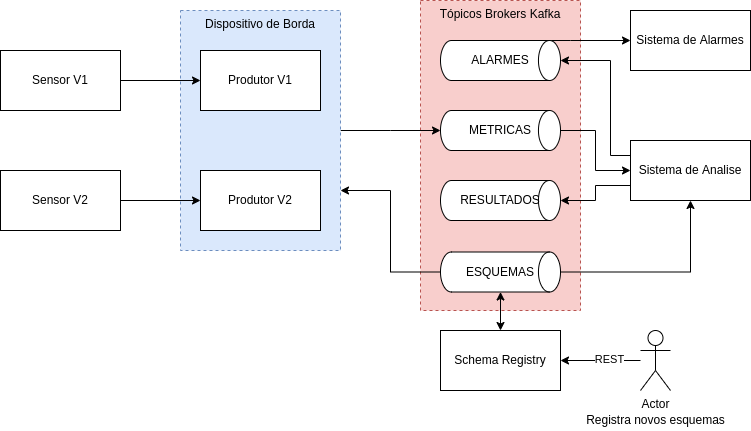
\includegraphics[width=0.8\textwidth]{images/fluxo_de_dados.png}
    \caption{Fluxo de Dados}
    \label{fig:fluxoDeDados}
\end{figure}

\subsection{Descrição dos Experimentos}
Para os testes práticos, foram criadas duas aplicações em Java, que utilizam a Producer e Consumer API. Utilizando variáveis de ambiente dentro dos contêineres e através das configurações de escala dos mesmos, é possível aumentar ou diminuir a quantidade de instâncias de cada aplicação de forma arbitrária.

Os testes foram conduzidos tentando levar os nós do Kafka a consumirem 100\% da capacidade da CPU disponível. O intuito era avaliar a quantidade de mensagens que este ambiente suportaria processar quando a CPU estivesse completamente saturada. Além disso, um aspecto importante é que a quantidade de memória também fosse suficiente para suportar a quantidade de mensagens em trânsito. A aplicação produtora de arquivos era escalada até o ponto de estresse e a aplicação consumidora mantida para avaliar quando a mesma se torna incapaz de ler a uma taxa maior ou igual à taxa de escrita, pois isso é o que passa a tornar a latência do sistema algo perceptível.

\subsection{Resultados}

\subsubsection{Throughput}

Como base para os experimentos, primeiro foi realizado o levantamento do desempenho de um \textit{broker}, quando não há nenhuma garantia de entrega, seja por arquivos duplicados ou perdas. Neste cenário, cada produtor era capaz de produzir aproximadamente 800 mensagens por segundo, e a quantidade de mensagens que eram despachadas para o \textit{broker} cresceu de forma quase que linear à medida que novos produtores foram introduzidos ao sistema (figura \ref{fig:g0a}). Isto demonstra que, dadas as necessidades de cada problema a ser resolvido, quando as garantias de entrega não precisam ser atendidas, até mesmo com um \textit{hardware} bastante limitado, os \textit{brokers} são capazes de processar uma quantidade massiva de mensagens. Este primeiro levantamento será utilizado como linha de base para avaliarmos os casos seguintes, em que buscamos realizar as entregas das mensagens de forma transacional, garantindo que as mensagens serão entregues uma e apenas uma vez.

\begin{figure}[ht]
    \centering
    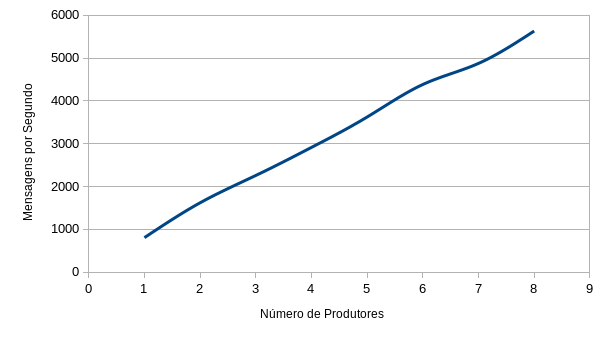
\includegraphics[width=0.8\textwidth]{images/graficos/g0a.png}
    \caption{1 \textit{BROKER} - 1 PARTIÇÃO}
    \label{fig:g0a}
\end{figure}

\begin{figure}[ht]
    \centering
    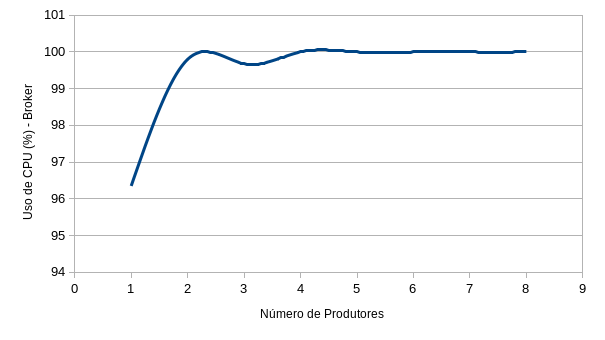
\includegraphics[width=0.8\textwidth]{images/graficos/g0b.png}
    \caption{1 \textit{BROKER} - 1 PARTIÇÃO}
    \label{fig:g0b}
\end{figure}
\clearpage

A primeira bateria de testes foi realizada com um \textit{broker} e uma partição (não há replicação neste cenário). Quando comparado ao caso de produtores não transacionais, podemos notar que a queda no volume de mensagens é vertiginosa, o que era de se esperar. Em contra partida, sempre em que houver falha na transmissão de dados, causando a perda ou duplicação dos dados, as transações serão revertidas, permitindo aos produtores realizar um novo envio no caso de perda ou cancelar um envio no caso de duplicidade. Para o número de produtores que o sistema foi capaz de manter, percebemos, inclusive, uma diminuição no uso dos recurso de CPU no \textit{broker}.

\begin{figure}[ht]
    \centering
    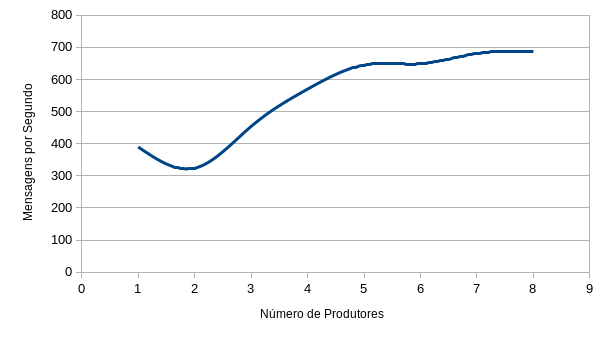
\includegraphics[width=0.8\textwidth]{images/graficos/g1a.png}
    \caption{1 \textit{BROKER} - 1 PARTIÇÃO}
    \label{fig:g1a}
\end{figure}

\begin{figure}[ht]
    \centering
    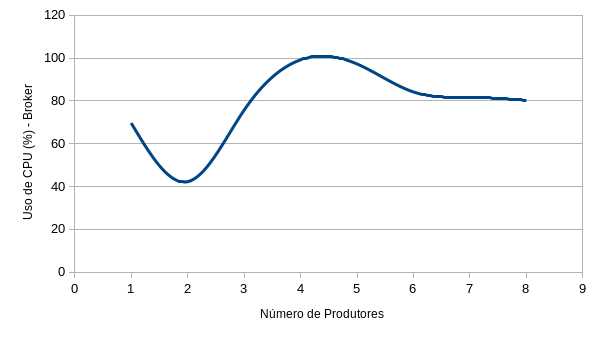
\includegraphics[width=0.8\textwidth]{images/graficos/g1b.png}
    \caption{1 \textit{BROKER} - 1 PARTIÇÃO}
    \label{fig:g1b}
\end{figure}
\clearpage

Ao aumentar o número de partições do tópico para 8, o volume de mensagens sofreu uma queda, se tornou maior quando o número de produtores estava entre 4 e 7, e se igualou ao caso anterior com 8 produtores. Neste caso, os produtores passam a despachar mensagens para todos os tópicos, e por serem transacionais, podem aproveitar do paralelismo para tentarem obter maior vazão, porém, há a necessidade de realizar o direcionamento dessas mensagens, o que pode acarretar em uma perda de desempenho.

\begin{figure}[ht]
    \centering
    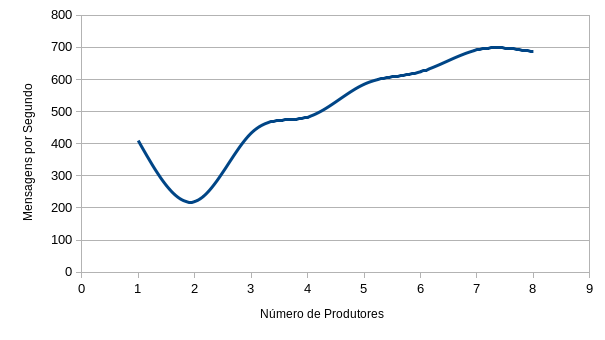
\includegraphics[width=0.8\textwidth]{images/graficos/g2a.png}
    \caption{1 \textit{BROKER} - 8 PARTIÇÕES}
    \label{fig:g2a}
\end{figure}

\begin{figure}[ht]
    \centering
    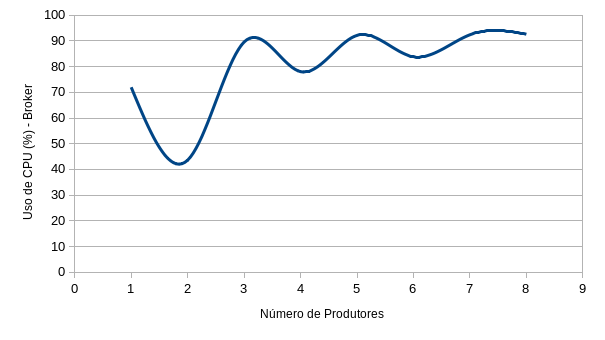
\includegraphics[width=0.8\textwidth]{images/graficos/g2b.png}
    \caption{1 \textit{BROKER} - 8 PARTIÇÕES}
    \label{fig:g2b}
\end{figure}
\clearpage

Com a utilização de 3 \textit{brokers} passamos a ter um desempenho inferior aos casos anteriores, o que era de se esperar, quando analisamos o desempenho de apenas um produtor. Com esta nova configuração, passamos a ter a comunicação com o \textit{broker} de forma distribuída. Esta configuração foi feita com 3 partições para garantir o uso efetivo de todos os \textit{brokers}, e ao mesmo tempo fosse certo que cada um abrigaria apenas uma praticão. Um produtor, precisa agora se comunicar com mais dois nós do Kafka, e com isso, tem uma maior demora de resposta do sistemas.

\begin{figure}[ht]
    \centering
    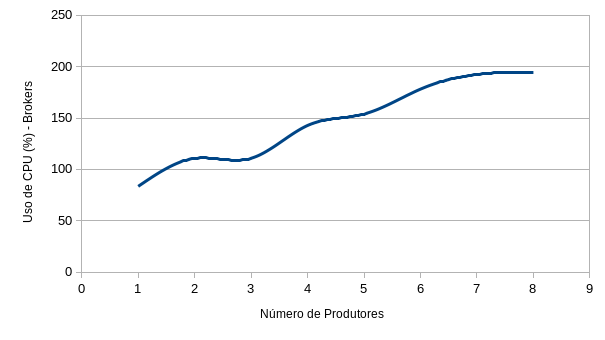
\includegraphics[width=0.8\textwidth]{images/graficos/g3b.png}
    \caption{3 \textit{BROKERS} - 3 PARTIÇÕES - 1 RÉPLICA}
    \label{fig:g3a}
\end{figure}

\begin{figure}[ht]
    \centering
    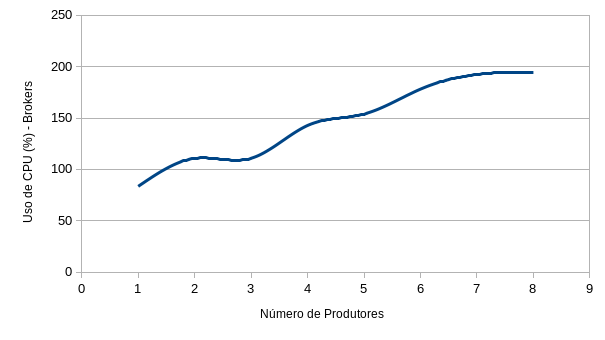
\includegraphics[width=0.8\textwidth]{images/graficos/g3b.png}
    \caption{3 \textit{BROKERS} - 3 PARTIÇÕES - 1 RÉPLICA}
    \label{fig:g3b}
\end{figure}
\clearpage

Em nosso último caso de testes, aumentamos o número de partições para 8, o número de réplicas para 3. Nesse caso, tivemos uma nova redução no número de mensagens que chegavam aos \textit{brokers} e um forte aumento na utilização de CPU, acarretado pelo maior número de  praticões sendo gerenciadas pelo \textit{cluster} e a maior troca de informação entre os próprios nós, uma vez que os \textit{brokers} passam a sincronizar as réplicas das partições para evitar perdas no caso de alguma falha no sistema de streaming.

\begin{figure}[ht]
    \centering
    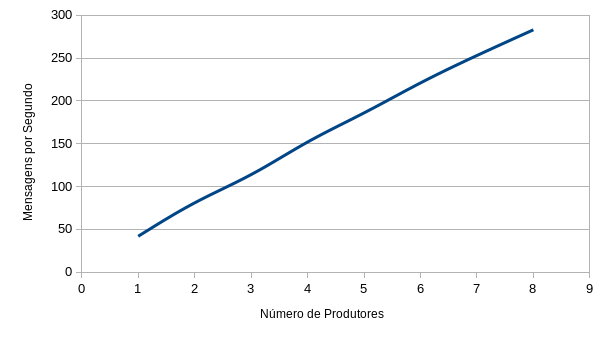
\includegraphics[width=0.8\textwidth]{images/graficos/g4a.png}
    \caption{3 \textit{BROKERS} - 8 PARTIÇÕES - 3 RÉPLICAS}
    \label{fig:g4a}
\end{figure}

\begin{figure}[ht]
    \centering
    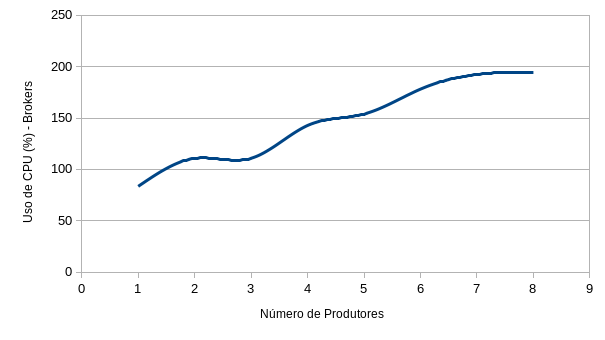
\includegraphics[width=0.8\textwidth]{images/graficos/g4b.png}
    \caption{3 \textit{BROKERS} - 8 PARTIÇÕES - 3 RÉPLICAS}
    \label{fig:g4b}
\end{figure}
\clearpage

\subsubsection{Latência}

A latência media foi realizada entre o despacho da mensagem por um produtor e o consumo da mesma por outra aplicação. Em todos os casos, não houve grande variação, sendo que o tempo entre a publicação no tópico pelo produtor e a resposta do consumidor a essa mesma mensagem sempre ficou em torno de 0.9 milisegundo.

\subsection{Análise}

Todas as medidas para garantir escalabilidade e resiliência ao sistema reduzem a capacidade de processamento imediato do sistema. Porém, dadas estas configurações, o sistema se mostra capaz de atender a uma 

Trabalhos futuros: Replicar a mesma infraestrutura em um cluster com: Raspberry Pi 4 B (4 GB)

\clearpage
%\newpage
\bibliographystyle{sbc}
\bibliography{sbc-template}

\end{document}